\documentclass[11pt,a4paper]{article}
\usepackage[T1]{fontenc}
\usepackage[utf8]{inputenc}
\usepackage{lmodern}
\usepackage[margin=2.15cm,top=2.1cm,bottom=2.1cm]{geometry}
\usepackage{microtype}
\usepackage{graphicx}
\graphicspath{{../report-figures/}{../results/plots/}{../results/user-interface/}}
\usepackage{booktabs,array,tabularx}
\usepackage{amsmath}
\usepackage{subcaption}
\usepackage[font=small,labelfont=bf]{caption}
\usepackage{listings}
\usepackage{xcolor}
\usepackage{tikz}
\usetikzlibrary{positioning,arrows.meta,fit}
\usepackage{enumitem}
\usepackage[hidelinks]{hyperref}
\usepackage{fancyhdr}
\usepackage{titlesec}

\setlist{itemsep=1pt,topsep=3pt,parsep=0pt}
\setlength{\parskip}{3pt}
\setlength{\parindent}{0pt}
\titlespacing*{\section}{0pt}{11pt}{4pt}
\titlespacing*{\subsection}{0pt}{7pt}{2pt}
\renewcommand{\arraystretch}{1.12}
\pagestyle{fancy}
\fancyhf{}
\renewcommand{\headrulewidth}{0.3pt}
\lhead{\small LIFELINE, group 41}
\rhead{\small DAA project, Iteration 2}
\cfoot{\small\thepage}
\setlength{\headheight}{14pt}

\lstdefinestyle{pseudo}{basicstyle=\ttfamily\footnotesize,columns=fullflexible,keepspaces=true,
  frame=single,framerule=0.3pt,rulecolor=\color{black!40},xleftmargin=2pt,xrightmargin=2pt,
  aboveskip=4pt,belowskip=4pt,showstringspaces=false,breaklines=true,mathescape=true}
\lstset{style=pseudo}

\newcommand{\cs}[1]{\texttt{#1}}
\newcolumntype{R}{>{\raggedleft\arraybackslash}X}

\begin{document}

%%%%%%%%%%%%%%%%%%%%%%%%%%%%%%%%%%%%%%%%%%%%%%%%%%%%%%% title page
\begin{titlepage}
\centering
\vspace*{1.2cm}

\includegraphics[width=3.2cm]{../report-figures/nu-logo.png}\\[8pt]
{\large National University of Computer and Emerging Sciences, Islamabad}\\[3pt]
{\large Design and Analysis of Algorithms, Iteration 2}\\[1.6cm]
{\Huge\bfseries LIFELINE}\\[6pt]
{\Large Choosing, building and measuring the algorithms of a relief-command engine}\\[1.4cm]
{\large Group 41}\\[10pt]
\begin{tabular}{lll}
Dur E Adan & 24I-3037 & Section C\\
Ayna Khan & 24I-0097 & Section C\\
Hamza Sardar & 24I-0089 & Section C\\
\end{tabular}\\[1.2cm]
\begin{minipage}{0.86\textwidth}
\textbf{Abstract.}
LIFELINE is a relief-command engine for a flood and earthquake scenario. This report describes the engine that group 41 built for six
decision problems: loading a truck (0/1 knapsack), planning routes, scheduling rescue windows, serving emergency alarms, planning a cable network, and
choosing matrix-chain products and drum cuts. For every problem the group implemented one primary algorithm and at least one baseline,
tested it against an independent reference and against planted faults, and measured it with a fixed protocol on pooled inputs of the master dataset.
The measured growth agrees with theory in most places: the knapsack table grows with slope 2.08 in the number of crates, the matrix-chain DP with slope 2.89, and a linear-scan queue
loses to a binary heap by a factor of 113 at 64\,000 alarms. In a few places theory and data disagree; the greedy rules for the knapsack and the drum cut are nearly optimal on the real data
although they are not optimal in theory. A seven-day campaign connects the modules on five master cases and three policies; all 105 daily records pass their output checks.
A newspaper-style web interface was added on top. The report ends with a ranked list of the three failure modes that worry the group most, and
with limitations that are stated openly, among them that all timings come from two laptops.
\end{minipage}
\vfill
{\small Repository: \url{https://github.com/ayna-khan/24I-3037-C_24I-0097-C_24I-0089-C}\\All numbers in this report are produced by the code in that repository and in the submitted folder.}
\end{titlepage}

%%%%%%%%%%%%%%%%%%%%%%%%%%%%%%%%%%%%%%%%%%%%%%%%%%%%%%% 1
\section{Introduction}
The project statement describes a district hit by floods and earthquakes. A command centre (HQ) has to decide, for seven days in a row, which crates go on the truck, which road the truck takes,
which rescue teams are staffed, and in which order emergency alarms are answered. In Iteration 1 the group generated and validated its own cases; in Iteration 2 the task
is to pick an algorithm for each problem, justify the pick with measurements, and connect the modules into one engine.

The group's six problems are (modules named as in the proposal): \textbf{A} relief inventory (0/1 knapsack), \textbf{B} route planning (shortest paths), \textbf{C} rescue scheduling (interval scheduling),
\textbf{D} emergency queue (priority queue), \textbf{F} network planning (minimum spanning tree) and \textbf{G} chains and cuts (matrix-chain order and drum cutting).
Everything is written in Python with the standard library; \cs{matplotlib} is used for the plots only.

The code, tests, results and this report are in the group's GitHub repository (\url{https://github.com/ayna-khan/24I-3037-C_24I-0097-C_24I-0089-C}); the same folder is submitted as the ZIP.

The report follows the order of the statement. Section~\ref{sec:data} describes the data and the pools. Section~\ref{sec:algo} gives the problem, the algorithms, their complexity and the key pseudocode
of each module, and states which choices of the proposal were kept. Section~\ref{sec:system} shows the architecture, Section~\ref{sec:tests} the tests, Section~\ref{sec:exp} the experiments and
the prediction log, and Section~\ref{sec:camp} the seven-day campaign. Section~\ref{sec:ui} shows the interface. Sections~\ref{sec:rec} to \ref{sec:work} give the recommendation, the limitations, the work division and the references.

%%%%%%%%%%%%%%%%%%%%%%%%%%%%%%%%%%%%%%%%%%%%%%%%%%%%%%% 2
\section{Data}\label{sec:data}
Only the course release \cs{master\_release\_v1} (2026-11-12) is used. It holds 3\,622 validated cases from 75 groups: 1\,429 of tier S, 1\,461 of tier M, 440 of tier L and 292 of tier X, spread over 20 CSV files
whose SHA-256 values are checked by the program (\cs{python -m src.cli --master MASTER verify}). A case is one disaster scenario with its locations, roads, crates, rescue windows, alarms, dimensions and price tables.
The group's seed is 41, so the samples take the cases at positions $41 \bmod 7 = 6, 13, 20,\dots$ of a tier, in the order of \cs{cases.csv}. The report says ``master order'' in this sense; the statement does not define it more closely, and this is one of the readings
that the group had to choose (Section~\ref{sec:limits}) \cite{stmt}.

\textbf{Case studies.} The six case studies are the six modules above, each run on its own table of the master data: crates for A, locations and roads for B and F, windows for C, alarms for D, and dimension lists and drum prices for G.
The five campaign cases are 1-06 (S), 1-26 (M), 2-40 (L), 2-48 (X, trap 48) and 4-47 (X, trap 47).

\textbf{Pooled instances.} A single case is too small for a growth experiment, so consecutive cases of one tier are joined, starting at the first case of the sample.
Crates are appended and the capacity of a pool is $\lfloor n\sum W_i / \sum n_i\rfloor$, which keeps the capacity per crate of the data (the statement does not fix it; this varies between 2.9 and 4.2 kg per crate).
Alarm ticks of a joined case are shifted past the last tick of the previous one, so the arrival rate stays at 1.2 to 1.8 alarms per tick. Rescue windows of the $i$-th case are shifted by $1440\,i$ minutes, so pooled cases never overlap in time.
Chains are concatenated dimension lists. A drum of length $L$ uses the first $L$ prices of one real table (case 12-47), because tables of different cases cannot be joined sensibly. Networks are never pooled; the growth runs for B and F use seven connected prefixes of one real graph (case 10-40, 16 to 1\,024 locations).
These choices keep the structure of real data but have a price: no experiment has thousands of windows inside one day, and the seven sizes of B and F are nested, not independent.

%%%%%%%%%%%%%%%%%%%%%%%%%%%%%%%%%%%%%%%%%%%%%%%%%%%%%%% 3
\section{Algorithm selection and design}\label{sec:algo}
Ties are broken by id ascending everywhere unless a rule below says otherwise. Broken input never turns into a plausible answer: it raises \cs{InvalidInputError} or returns a status (\cs{INVALID}, \cs{EMPTY}, \cs{NO\_ROUTE}, \cs{TOO\_LARGE}), depending on the module.
Table~\ref{tab:algos} summarises the choices; the following subsections give details.

\begin{table}[t]
\centering\small
\caption{Primary algorithm and baselines of each module, with the status of the proposal choice.}\label{tab:algos}
\begin{tabularx}{\textwidth}{@{}l>{\raggedright\arraybackslash}p{2.6cm}>{\raggedright\arraybackslash}p{3.7cm}>{\raggedright\arraybackslash}p{2.5cm}X@{}}
\toprule
 & Primary & Baselines & Time of primary & Proposal\\
\midrule
A & DP over capacity & ratio greedy; brute force & $O(nW)$ & kept; table width cut to $\min(W,\text{total weight})$\\
B & heap Dijkstra, BFS & Bellman-Ford; BFS as cost policy & $O((V+E)\log V)$ & kept; array Dijkstra not implemented\\
C & earliest finish (count); weighted-interval DP (value) & plain $O(n^2)$ DP; brute force; greedy on value & $O(n\log n)$ & kept; greedy on value added as a baseline\\
D & binary heap & linear scan; FIFO only for comparison & $O(m\log m)$ & kept; ten-bucket queue not implemented\\
F & Kruskal with union-find & heap Prim & $O(E\log E)$ & kept; Bor\r{u}vka and array Prim not implemented\\
G & bottom-up DP (chain, drum) & memoised recursion; greedy cut; brute force & $O(n^3)$, $O(L^2)$ & kept; tie rules and \cs{TOO\_LARGE} added\\
\bottomrule
\end{tabularx}
\end{table}

\subsection{Module A: relief inventory}
\textbf{Problem.} Given $n$ crates with whole-number weight $w_i$ and value $v_i$ and a truck capacity $W$, choose a set of crates of total weight at most $W$ with the largest total value.
On day $d$ the values change by category (tools $\times2$ on day 2, food $\times2$ on day 3, medicine $\times3$ on day 5).
\textbf{Algorithms.} The primary method is the DP over the capacity \cite{clrs}, $O(nW)$ time and $n(W+1)$ bytes for a back-tracking table; the baselines are the ratio-greedy rule \cite{mt} ($O(n\log n)$, exact fractions compared by cross-multiplication, our own merge sort) and brute force
over Gray-code subsets ($O(2^n)$, refused above $n=22$). The total value is unique; among equal-value sets the back-tracking prefers earlier crates.
\textbf{Retained or changed.} Retained. The table width was reduced to $\min(W,\text{total weight})$.

\begin{lstlisting}[caption={Module A, DP with back-tracking (key steps).},captionpos=b,label=lst:a]
best[0..W] = 0;  keep[i][c] = false for all i, c
for each crate i with w[i] <= W and v[i] > 0:
    for c = W downto w[i]:
        if best[c - w[i]] + v[i] > best[c]:
            best[c] = best[c - w[i]] + v[i];  keep[i][c] = true
c = W;  for i = n downto 1:  if keep[i][c]: take crate i;  c = c - w[i]
\end{lstlisting}

\subsection{Module D: emergency queue}
\textbf{Problem.} Alarms have an arrival tick and a priority from 1 to 10. One alarm is released per tick; the released one is the most urgent among those present (priority descending, arrival ascending, id ascending).
\textbf{Algorithms.} Primary: a binary min-heap \cite{clrs} on the key $(-\text{priority},\text{tick},\text{id})$, $O(m\log m)$. Baseline: a linear scan of all waiting alarms at every tick, $O(m\cdot\text{backlog})$, which must give exactly the same release order.
First-come-first-served is implemented only to show what the urgency order buys; it is not a solution of the module. \textbf{Retained or changed.} Retained; the ten-bucket queue named in the proposal was not built.

\begin{lstlisting}[caption={Module D, release loop with the heap.},captionpos=b,label=lst:d]
now = 0;  i = 0                                  // alarms sorted by arrival tick
while i < m or heap not empty:
    if heap is empty: now = max(now, arrival[i])
    while i < m and arrival[i] <= now: push(heap, key(alarm i));  i = i + 1
    a = pop_min(heap);  release a at tick now;  now = now + 1
\end{lstlisting}

\subsection{Module C: rescue scheduling}
\textbf{Problem.} A window has a start, a finish and a value; two windows are compatible when one starts at or after the finish of the other. On day $d$ the window with $(\text{id}+d)\bmod 5=0$ is unavailable.
Choose compatible windows with the largest count, or the largest total value. \textbf{Algorithms.} For the count the earliest-finish rule is optimal by an exchange argument \cite{kt} ($O(n\log n)$). For the value, weighted-interval DP \cite{kt}
with $p(i)$ found by binary search, $O(n\log n)$ (Listing~\ref{lst:c}). Baselines: the plain $O(n^2)$ DP, brute force up to 22 windows, and the earliest-finish rule on the value objective, which the group kept as a measured baseline
because it shows what ignoring the values costs. \textbf{Retained or changed.} Retained; the greedy-on-value baseline and the statuses \cs{EMPTY} and \cs{INVALID} were added so that a day without windows does not crash the campaign.

\begin{lstlisting}[caption={Module C, weighted-interval DP with binary search.},captionpos=b,label=lst:c]
sort windows by (finish, id)
for i = 1 to n:
    p[i] = number of earlier windows with finish <= start[i]        // binary search
    best[i] = max(best[i-1], best[p[i]] + value[i])                  // strict: ties skip i
i = n;  while i > 0:  if best[i] != best[i-1]: take window i;  i = p[i]  else  i = i - 1
\end{lstlisting}

\subsection{Module G: chains and cuts}
\textbf{Problem.} \emph{Chain:} for dimensions $p_0,\dots,p_n$ find the bracketing of the product $A_1\cdots A_n$ with the fewest scalar multiplications. \emph{Drum:} for a price list of lengths $1,\dots,L$ cut a drum of length $L$ into pieces of maximal total price.
\textbf{Algorithms.} Both use bottom-up DP with a split table \cite{clrs}: $\text{cost}[i][j]=\min_k \text{cost}[i][k]+\text{cost}[k{+}1][j]+p_{i-1}p_kp_j$, $O(n^3)$ time with $(n^3-n)/6$ split candidates; $\text{best}[l]=\max_k \text{price}(k)+\text{best}[l-k]$, $O(L^2)$ time with $L(L+1)/2$ candidates.
Baselines: the memoised recursion (same recurrences, but as deep as $n$ or $L$, so it runs in a helper thread with a large stack), the greedy cut by price per length for the drum ($O(L\log L)$, not optimal), and brute force (Catalan$(n-1)$ bracketings for $n\le12$, $2^{L-1}$ cuts for $L\le20$). A faster chain algorithm of Hu and Shing \cite{hs} exists and was not implemented.
Fixed tie rules make dp, memo and brute force return exactly the same answer. \textbf{Retained or changed.} Retained; the tie rules, the status \cs{TOO\_LARGE} and the helper thread were added so that a deep recursion ends in an answer or a status.

\subsection{Modules B and F: routes and networks}
\textbf{B.} A directed step costs the minutes of the road plus the penalty of the destination, all positive. Heap Dijkstra \cite{dij} computes the cheapest route and all distances, $O((V+E)\log V)$; BFS gives reachability and the fewest-roads route.
The baselines are early-stopping Bellman-Ford, $O(VE)$, and BFS used as a travel-cost policy. \textbf{F.} Kruskal \cite{kru} with union by size and path compression \cite{tar}, $O(E\log E+E\alpha(V))$, is the primary method and heap Prim the independent check; a disconnected map gives a forest.
The proposal choices were retained; array Dijkstra, array Prim and Bor\r{u}vka were not implemented.

%%%%%%%%%%%%%%%%%%%%%%%%%%%%%%%%%%%%%%%%%%%%%%%%%%%%%%% 4
\section{System design and implementation}\label{sec:system}
The code is split into one file per decision module, a shared loader and validation layer, a campaign coordinator and two front doors (command line and local HTTP API), as in Figure~\ref{fig:arch}.
The decision modules know nothing about files or the calendar: they receive records and return a plan with a status and an operation count. The loader streams only the rows of the requested cases from the large CSV files and validates schemas, integer cells, unique ids,
positive costs and closure references. The coordinator transforms the base data for each day of the official calendar (Section~\ref{sec:camp}), calls A, B, C and D, and on day 7 also F and G, and then \emph{checks} every output against the rules of the problem
(open roads, capacity, compatibility of windows, release order) instead of trusting it. The baseline policy calls the same entry points with the baseline methods.

\begin{figure}[t]
\centering
\resizebox{\textwidth}{!}{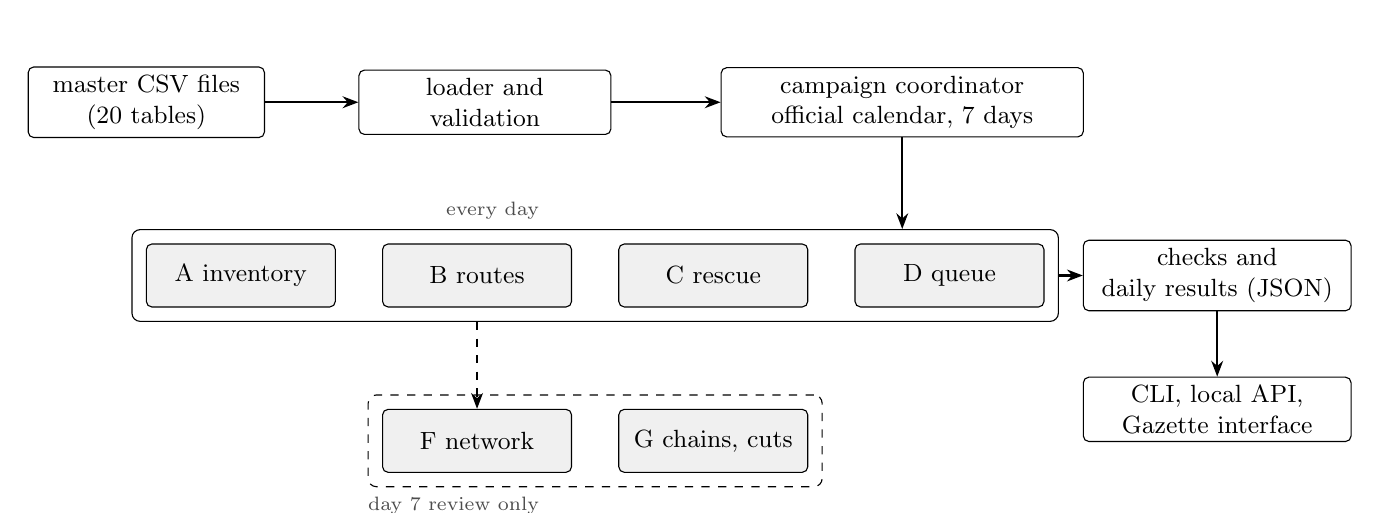
\begin{tikzpicture}[font=\small,
  box/.style={draw,rounded corners=2pt,minimum height=8mm,align=center,inner sep=3pt},
  mod/.style={box,fill=black!6,minimum width=2.4cm},
  arr/.style={-{Stealth[length=2mm]},thick}]
\node[box,minimum width=3cm] (csv) at (0,0) {master CSV files\\(20 tables)};
\node[box,minimum width=3.2cm] (load) at (4.3,0) {loader and\\validation};
\node[box,minimum width=4.6cm] (camp) at (9.6,0) {campaign coordinator\\official calendar, 7 days};
\draw[arr] (csv)--(load); \draw[arr] (load)--(camp);
\node[mod] (A) at (1.2,-2.2) {A inventory};
\node[mod] (B) at (4.2,-2.2) {B routes};
\node[mod] (C) at (7.2,-2.2) {C rescue};
\node[mod] (D) at (10.2,-2.2) {D queue};
\node[mod] (F) at (4.2,-4.3) {F network};
\node[mod] (G) at (7.2,-4.3) {G chains, cuts};
\node[draw,rounded corners=3pt,inner sep=5pt,fit=(A)(B)(C)(D),label={[font=\scriptsize,text=black!70]above left:every day}] (daily) {};
\node[draw,dashed,rounded corners=3pt,inner sep=5pt,fit=(F)(G),label={[font=\scriptsize,text=black!70]below left:day 7 review only}] (d7) {};
\draw[arr] (camp.south) -- (camp.south |- daily.north);
\draw[arr,dashed] (daily.south -| F.north) -- (F.north);
\node[box,minimum width=3.4cm] (out) at (13.6,-2.2) {checks and\\daily results (JSON)};
\node[box,minimum width=3.4cm] (ui) at (13.6,-3.9) {CLI, local API,\\Gazette interface};
\draw[arr] (daily.east)--(out); \draw[arr] (out)--(ui);
\end{tikzpicture}}
\caption{Architecture and data flow. The coordinator feeds each day's transformed input to the modules and checks their outputs; F and G run only in the day-7 planning review.}\label{fig:arch}
\end{figure}

Each module has the same small interface (\cs{solve(input, method, deadline)}), so the measurement harness, the campaign and the tests call every method the same way. The harness gives every run a deadline; a run that passes 300~s raises
\cs{TimeBudgetExceeded} and is recorded as DNF. A local server (\cs{src/server.py}, bound to 127.0.0.1) exposes the modules as JSON endpoints, and the interface of Section~\ref{sec:ui} reads only from it.

%%%%%%%%%%%%%%%%%%%%%%%%%%%%%%%%%%%%%%%%%%%%%%%%%%%%%%% 5
\section{Testing}\label{sec:tests}
\textbf{Strategy.} Each module has (i) unit tests of the rules and edge cases (empty input, touching windows, a crate that exactly fills the truck, equal priorities, duplicate ids), (ii) an independent \emph{reference} that never imports the shipped code
(for example a Gray-code brute force for A, \cs{sorted} for D, an interval-subset enumeration for C, plain recursion for G), compared against the shipped methods on the fixtures and on random small inputs, (iii) integration tests of the campaign and the HTTP API,
and (iv) fault-injection tests. The full suite has 223 tests (about 100~s) and passes, with two skipped tests, the slow fault-injection runs of C and G, which are run separately (Table~\ref{tab:fault}).

\textbf{Fault injection.} For each module the repository is copied, one realistic bug is planted in the shipped source (a wrong tie rule, \texttt{<} instead of \texttt{<=} at a boundary, a missing validation check, a back-tracking that steps the wrong way,
a time budget that is never checked) and the module's tests must fail. Table~\ref{tab:fault} shows that all 59 planted faults are caught.

\begin{table}[t]
\centering\small
\caption{Planted faults and unit tests per module.}\label{tab:fault}
\begin{tabular}{@{}lrrl@{}}
\toprule
Module & Unit tests (file) & Planted faults & Caught\\
\midrule
A and D & 25 + 25 & 10 & 10 of 10\\
C & 54 & 14 & 14 of 14\\
G & 63 & 20 & 20 of 20\\
B and F (with campaign) & 22 + 9 & 15 & 15 of 15\\
\bottomrule
\end{tabular}
\end{table}

\textbf{Failures and their diagnosis.} The group found three real problems. First, a test helper file contained the wrong module (it imported an inventory reference where a fixture builder was expected), which made every test of the test package fail with an
import error; the fix was to restore the helper. Second, one fault of C (back-tracking that steps back one window instead of jumping to $p(i)$) was reported as ``not applied'' on a Windows checkout: the planted text contains line feeds, but a Windows checkout has CRLF line endings,
so the text was never found. The injector now normalises line endings before it plants the fault and the fault is caught. Third, a memoised recursion that is as deep as the input (2\,000 calls for a drum of $L=2000$) must end in an answer or a status and never in a crash, which is why G runs it in a helper thread and returns \cs{TOO\_LARGE} above depth 20\,000.
One fault of B is a relaxation loop that never ends; it is caught by a five-second timeout, not by a failing assertion.

%%%%%%%%%%%%%%%%%%%%%%%%%%%%%%%%%%%%%%%%%%%%%%%%%%%%%%% 6
\section{Experiments and analysis}\label{sec:exp}
\textbf{Protocol.} One discarded warm-up run, then five timed runs; the report uses the median and the interquartile range (IQR). Garbage collection is off while a run is timed, data loading is excluded, and runs under 10~ms are timed as a batch.
Growth is fitted by least squares on at least five sizes (log-log for polynomial growth, semi-log for exponential growth) with a 95\,\% confidence interval from the $t$ distribution and $R^2$. Operation counts follow the families of the statement
(for example table cells for the DP, key comparisons plus moves for the heap) and are written in \cs{results.csv} (204 rows: A 39, B 21, C 43, D 20, F 14, G 67). Memory is measured with \cs{tracemalloc}.
Module A and D numbers come from Ayna's laptop (Windows 11, CPython 3.13.7); C and G from Adan's laptop (Windows 10, CPython 3.14.6); B and F from Hamza's computer (Windows 11, AMD CPU with 16 logical processors, CPython 3.14.3). Absolute times are therefore only comparable inside one module.

\textbf{A disturbed run.} During the first full run of A and D the speed of Ayna's laptop changed: the time per DP cell moved between 139 and 398~ns. Rounds 1 and 3 were repeated with the charger connected and the power mode on best performance (about 85~ns per cell).
Rounds 2 and 4 were not repeated; their absolute times (brute force at $n=20$, 256\,000 alarms) are less reliable than the operation counts, which are exact. The 6\,400-crate run still changed speed during its five timed runs (IQR 8.8~s).

\subsection{Growth against theory}
Table~\ref{tab:fits} lists the main fits. The counted operations follow theory closely. Times follow the operations with slope near 1 (A: $1.07\pm0.14$, C: $0.97\pm0.09$, G: $0.98$), so the operation counts explain the times.
The fitted time slope of the A DP (2.22) is above the operation slope (2.08) because of the disturbed 6\,400-crate point; without it the slope is $2.05\pm0.21$.

\begin{table}[t]
\centering\small
\caption{Empirical growth against theory (log-log slope of the median time with 95\,\% interval, against the theoretical exponent).}\label{tab:fits}
\begin{tabularx}{\textwidth}{@{}llXrr@{}}
\toprule
Module & Method and size range & Experiment & Slope & Theory\\
\midrule
A & DP, 200 to 6\,400 crates & A-scale-n & $2.22\pm0.28$ & 2\\
A & DP, $W$ grows, $n=1600$ & A-scale-W & $0.86\pm0.27$ & 1\\
D & heap, 250 to 64\,000 alarms & D-scale-m & $1.12\pm0.11$ & $\approx1$ ($m\log m$)\\
D & linear scan, same sizes & D-scale-m & $1.96\pm0.05$ & 2\\
C & greedy, 47 to 3\,000 windows & C-scale-n & $1.07\pm0.28$ & $\approx1$\\
C & DP with binary search & C-scale-n & $1.26\pm0.10$ & $\approx1$\\
C & plain $O(n^2)$ DP & C-scale-n & $1.85\pm0.21$ & 2\\
G & chain DP, 10 to 640 matrices & G-chain-n & $2.89\pm0.15$ & 3\\
G & drum DP, 63 to 2\,000 & G-drum-L & $2.03\pm0.10$ & 2\\
G & greedy cut, same sizes & G-drum-L & $1.16\pm0.03$ & $\approx1$\\
\bottomrule
\end{tabularx}
\end{table}

\begin{figure}[t]
\centering
\begin{subfigure}{0.48\textwidth}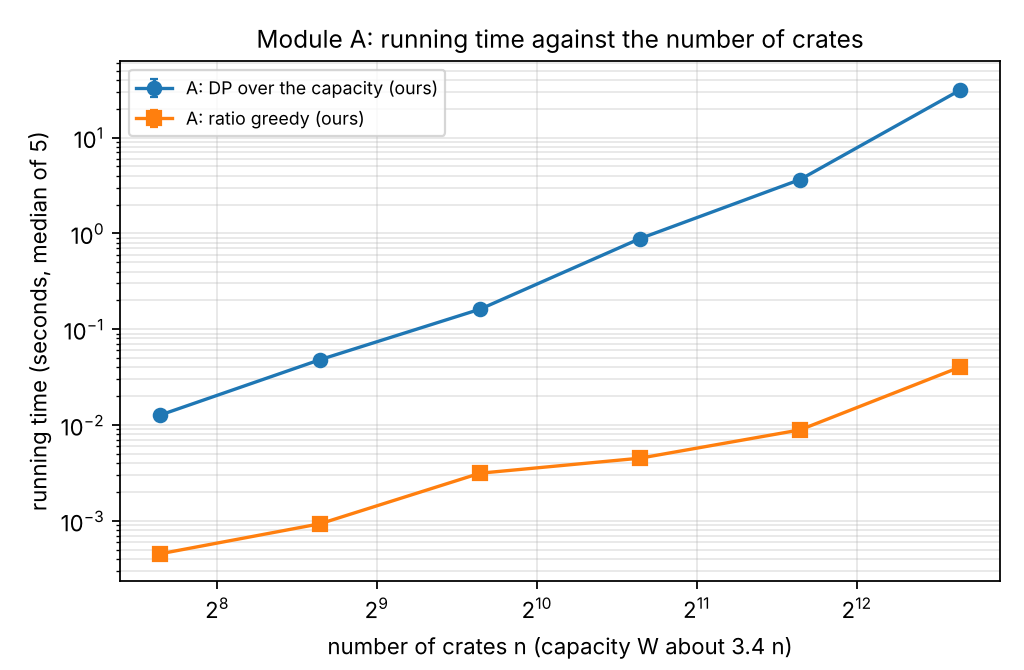
\includegraphics[width=\linewidth]{A-time-vs-n.png}\caption{Module A, time against $n$.}\end{subfigure}\hfill
\begin{subfigure}{0.48\textwidth}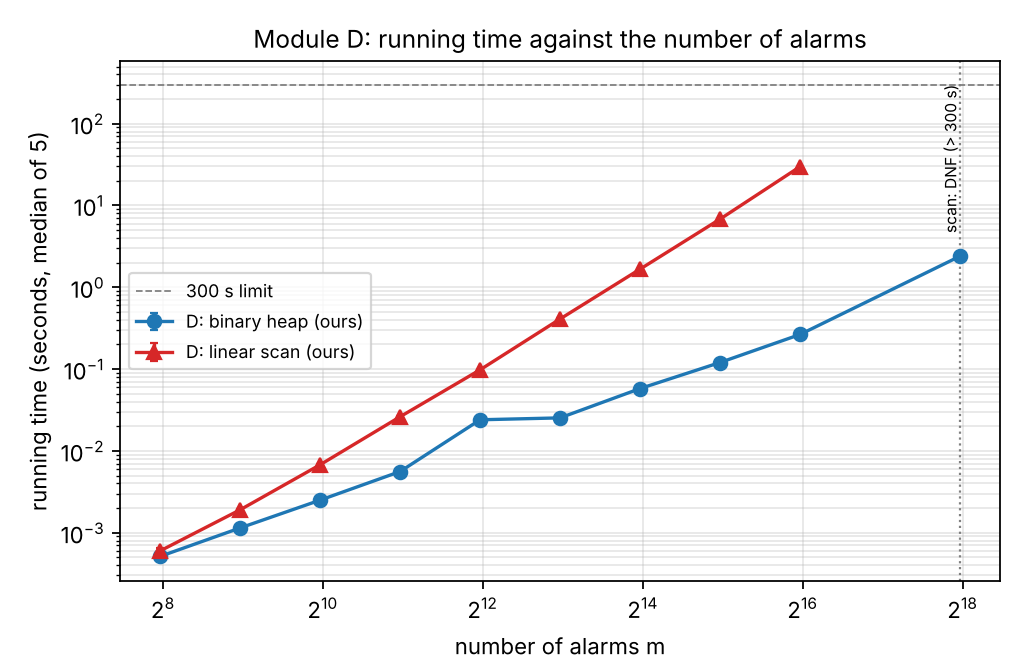
\includegraphics[width=\linewidth]{D-time-vs-m.png}\caption{Module D, time against $m$; the dashed line is 300~s.}\end{subfigure}\\[4pt]
\begin{subfigure}{0.48\textwidth}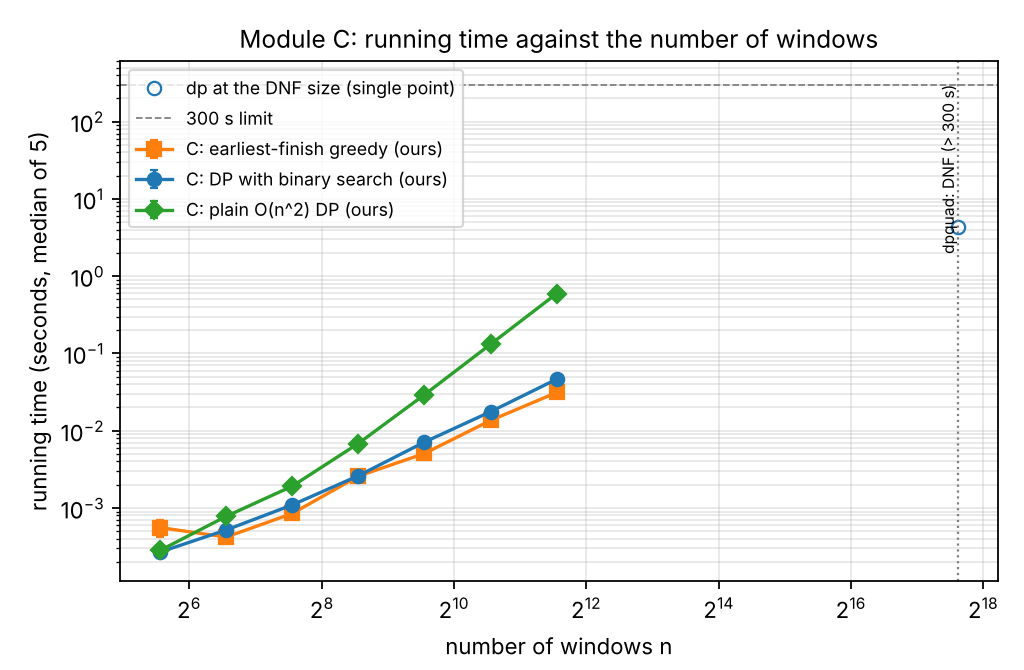
\includegraphics[width=\linewidth]{C-time-vs-n.png}\caption{Module C, time against $n$.}\end{subfigure}\hfill
\begin{subfigure}{0.48\textwidth}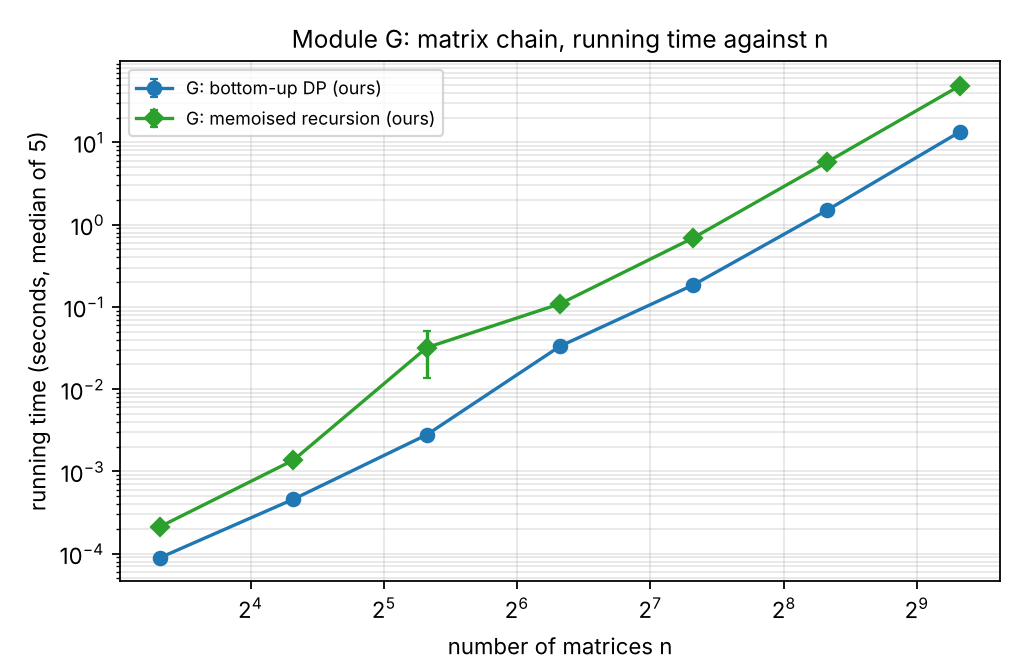
\includegraphics[width=\linewidth]{G-chain-time-vs-n.png}\caption{Module G, matrix chain.}\end{subfigure}
\caption{Median running time against input size, log-log, bars are the IQR.}\label{fig:growth}
\end{figure}

\subsection{Algorithms against their baselines}
\textbf{A.} At 6\,400 crates the DP needs 31.3~s (161 million cells) and the greedy rule 40~ms, so greedy is about 800 times faster. The DP buys value: it matches the claimed optimum in 20 of 20 tier S cases, while greedy is optimal in only 7 of 20 tier S and 7 of 20 tier M cases.
On the trap-47 cases greedy reaches 56\,\% of the optimum on average (Figure~\ref{fig:quality}a). On tiers M and L the loss is only 0.2\,\% and 0.01\,\%. Brute force doubles per crate (base 2.02, interval 1.94 to 2.11) and the DP is 878 times faster at $n=20$ (0.67~ms against 585~ms; round 2, slower run).

\textbf{D.} The scan is 1.2 times slower than the heap at 250 alarms, 29 times at 16\,000 and 113 times at 64\,000 (0.26~s against 29.8~s). At 256\,000 alarms the scan did not finish in 300~s (DNF) and the heap needed 2.4~s (a repeat is expected to give about 1.2~s, since this round came from the slow run).
The urgency order and FIFO have the same mean wait for all alarms, but priority 9 and 10 alarms wait 1.5 ticks under the heap against 639 under FIFO on tier L.

\textbf{C.} At 3\,000 windows greedy takes 31~ms, the DP 46~ms and the plain DP 0.60~s (13 times the DP; it examines exactly $n(n-1)/2$ pairs). At 200\,000 windows the DP needs 4.4~s while the plain DP is a DNF. Greedy is optimal for the count in 62 of 62 cases, but for the value it gives up 16\,\% (S), 23\,\% (M), 26\,\% (L) and 28\,\% (X) on average, and 73\,\% in the worst small case (Figure~\ref{fig:quality}b).
Brute force grows by 1.95 per window and the DP is 3\,900 times faster at $n=20$.

\textbf{G.} At 640 matrices the DP needs 13.4~s and the memoised recursion 48.7~s (3.6 times), with identical candidate counts; for the drum at $L=2000$ the DP takes 0.35~s, the recursion 1.17~s and greedy 13.8~ms. The greedy cut is optimal in 61 of 62 cases (worst 0.977 of the optimum) although it has no guarantee. Multiplying from left to right costs 4.5 to 16.9 times the optimum on average.

\textbf{B and F.} Dijkstra and Bellman-Ford agree on the cost in all 867 sampled target and wave checks. At 1\,024 locations Dijkstra takes 11.8~ms, Bellman-Ford 16.7~ms and BFS 10.2~ms, but BFS finds routes up to 20 times as expensive as the best one.
Kruskal and Prim agree on the forest cost in all 289 checks; at 1\,024 locations the times are 17.0 and 19.0~ms (ratio 1.11). That difference is small and specific to this network, so the group does not claim that Kruskal always wins.

\begin{figure}[t]
\centering
\begin{subfigure}{0.48\textwidth}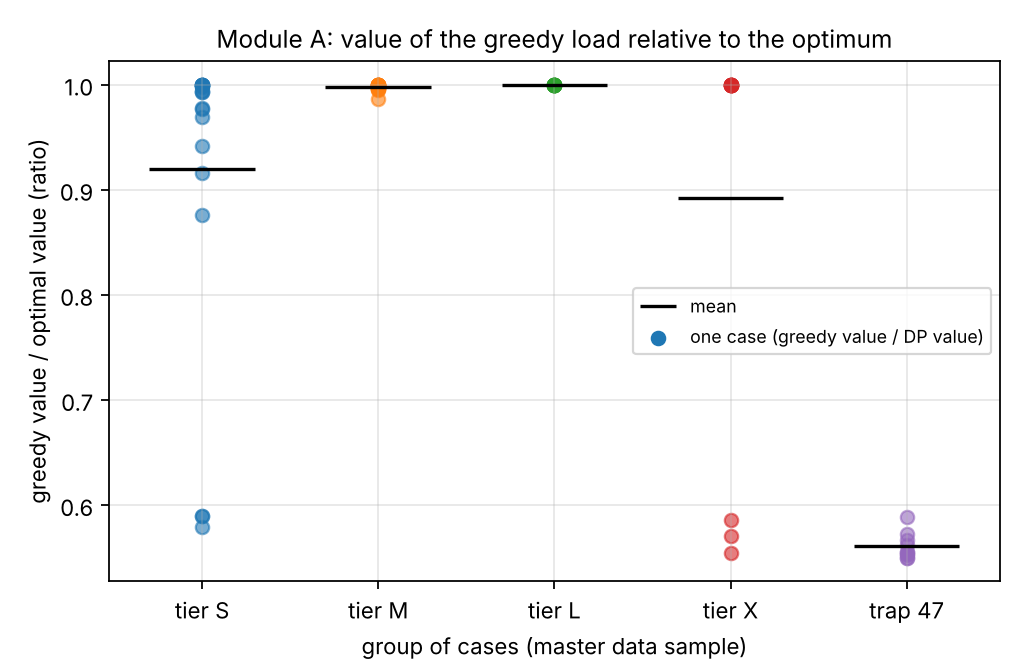
\includegraphics[width=\linewidth]{A-greedy-quality.png}\caption{A: greedy value / optimal value.}\end{subfigure}\hfill
\begin{subfigure}{0.48\textwidth}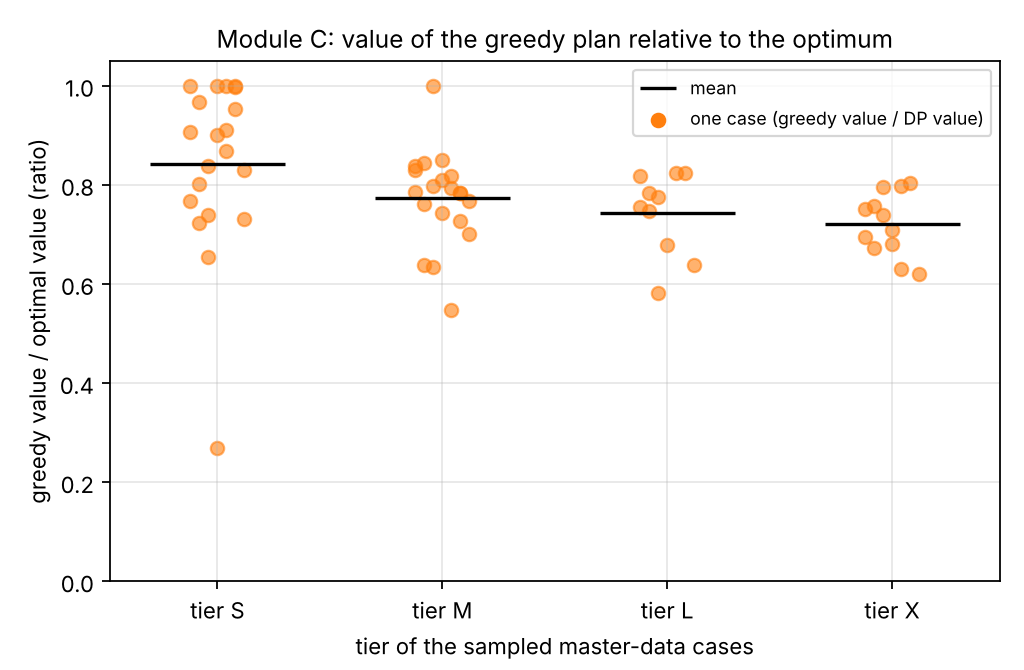
\includegraphics[width=\linewidth]{C-greedy-quality.png}\caption{C: greedy value / optimal value.}\end{subfigure}
\caption{Quality of the greedy rules on the sampled cases of each tier. The black bars are means.}\label{fig:quality}
\end{figure}

\subsection{Prediction log against outcomes}
Before every round the group wrote numeric predictions with tolerances into \cs{prediction\_log.md} and checked them afterwards with a script. Table~\ref{tab:pred} shows the result: 131 of 143 predictions fall inside their interval.
The log also states plainly where the commit order does not prove the order of events (for A and D the results were committed three minutes before the log).

\begin{table}[t]
\centering\small
\caption{Predictions against measurements.}\label{tab:pred}
\begin{tabularx}{\textwidth}{@{}lrrX@{}}
\toprule
Module & Predictions & Inside interval & Missed (examples)\\
\midrule
A, D & 31 & 27 & A DP time at 6\,400 crates (14~s predicted, 31.3~s); brute force at $n=20$; scan extrapolation at 256\,000\\
C & 37 & 31 & loss of greedy on the value (predicted 30 to 42\,\%, measured 16 to 28\,\%); greedy count at 3\,000\\
G & 48 & 46 & greedy drum optimal in 98\,\% of cases (predicted 85\,\%); left-to-right chain ratio (4.5, predicted 1.35)\\
B, F & 23 & 23 & none\\
Campaign & 4 & 4 & none\\
\bottomrule
\end{tabularx}
\end{table}

The misses are instructive. Two come from the speed change of the laptop (A and D). The three greedy-quality misses show that the data are kinder to greedy rules than the textbook worst cases suggest for the drum, and harsher than guessed for the chain.
The prediction that the greedy loss on windows would be 30 to 42\,\% was simply too pessimistic; the loss is large, just not that large.

%%%%%%%%%%%%%%%%%%%%%%%%%%%%%%%%%%%%%%%%%%%%%%%%%%%%%%% 7
\section{Campaign results}\label{sec:camp}
\textbf{The calendar.} The campaign implements Project Statement section 7.4. Every day starts at HQ and applies its change to the \emph{base} data, never to the previous day: day 2 (storm) multiplies minutes by $3/2$ rounded up, doubles the tool values, adds an alarm of priority 9 and closes wave 0; day 3 doubles food and closes wave 1;
day 4 doubles penalties of at least 2 and closes wave 2; day 5 triples medicine, adds an alarm of priority 10 and closes wave 3; day 6 (flood) closes the union of all waves; day 7 is an evacuation without loading, again on the union.
The destinations rotate over targets 0, 1, 2. Rescue windows with $(\text{id}+\text{day})\bmod5=0$ are unavailable. The wave index wraps modulo the number of waves.

\textbf{Policies.} The \emph{optimized} policy uses the shipped methods (DP loading, Dijkstra, the DP or greedy of C, the heap). The \emph{algorithm baseline} uses the baseline method of each module (ratio-greedy loading, Bellman-Ford, the plain quadratic DP for rescue, the linear scan), and the \emph{simple} policy uses
fewest-roads routes, ratio-greedy loading, the earliest-finish rule on the value objective and first-come-first-served alarms. The same input is used for all three. The measures of section 7.4 are kept as separate numbers; no combined score is invented.

\begin{table}[t]
\centering\small
\caption{Seven-day results of the optimized policy and the differences to the two comparison policies. "Base.\ delivered" is the delivered value of the baseline policy; delivered value counts the days 1 to 6 on which the destination is reachable.}\label{tab:camp}
\setlength{\tabcolsep}{4pt}
\begin{tabularx}{\textwidth}{@{}llRRRRRR@{}}
\toprule
Case & Tier & Delivered & Base.\ deliv. & Route cost & Unreach. days & Rescue value & Urgent wait opt./simple\\
\midrule
1-06 & S & 4\,631 & 4\,574 & 388 & 2 & 2\,401 & 0.13 / 2.4\\
1-26 & M & 13\,239 & 13\,207 & 591 & 1 & 14\,880 & 0.17 / 110.1\\
2-40 & L & 16\,871 & 16\,865 & 13\,339 & 6 & 25\,008 & 0.08 / 366.1\\
2-48 & X & 82\,113 & 82\,090 & 61 & 2 & 27\,289 & 0.11 / 376.0\\
4-47 & X & 1\,200 & 712 & 2\,490 & 1 & 13\,876 & 0.07 / 387.3\\
\bottomrule
\end{tabularx}
\end{table}

All 105 daily policy records (5 cases, 3 policies, 7 days) passed their output checks, and exact references (Bellman-Ford distances, quadratic rescue totals, urgency scans, Prim trees, memoised G) agree with the shipped methods on the same inputs.
Table~\ref{tab:camp} shows what the choices buy. The exact loading of A is never worse than greedy and clearly better on the hostile cases: on trap 47 the DP delivers 1\,200 over the campaign against 712 for greedy (on a single normal day 198 against 113, or 57\,\% of the optimum).
The urgency order keeps the mean wait of priority 9 and 10 alarms below 0.2 ticks, against 2.4 to 387 ticks for the simple policy. On trap 48 the fewest-roads route costs 64 and the cheapest costs 12, 5.3 times as much, so BFS is not a substitute for Dijkstra.
The simple policy loses 17 to 34\,\% of the rescue value. Route cost and rescue value are identical between the optimized and the baseline policy, as they must be, because the baselines of B and C are exact methods that are only slower.
Days 6 and 7 close every wave, and in several cases the destination is then cut off: between one and six unreachable days per case (case 2-40 has six). The engine reports \cs{NO\_ROUTE} and skips the trip instead of inventing a route.

\begin{table}[t]
\centering\footnotesize\setlength{\tabcolsep}{3.5pt}
\caption{Daily outcomes of the optimized policy on case 1-06 (seven locations, 19 crates, capacity 82; program output of \cs{python -m src.cli campaign}). Urgent wait is the mean wait of alarms of priority 9 and 10.}\label{tab:daily}
\begin{tabular}{@{}rlrrlrrrr@{}}
\toprule
Day & Event & Target & Closed roads & Trip & Route cost & Load value & Rescue value & Urgent wait\\
\midrule
1 & Normal & 4 & 0 & OK & 84 & 826 & 342 & 0.000\\
2 & Storm & 3 & 1 & OK & 48 & 843 & 304 & 0.333\\
3 & Food shortage & 1 & 1 & OK & 91 & 1\,310 & 365 & 0.000\\
4 & Dangerous area & 4 & 1 & OK & 132 & 826 & 353 & 0.000\\
5 & Medical emergency & 3 & 1 & OK & 33 & 826 & 391 & 0.333\\
6 & Flood & 1 & 3 & NO\_ROUTE & -- & -- & 342 & 0.000\\
7 & Evacuation & 4 & 3 & NO\_ROUTE & -- & -- & 304 & 0.000\\
\bottomrule
\end{tabular}
\end{table}

\begin{figure}[t]
\centering
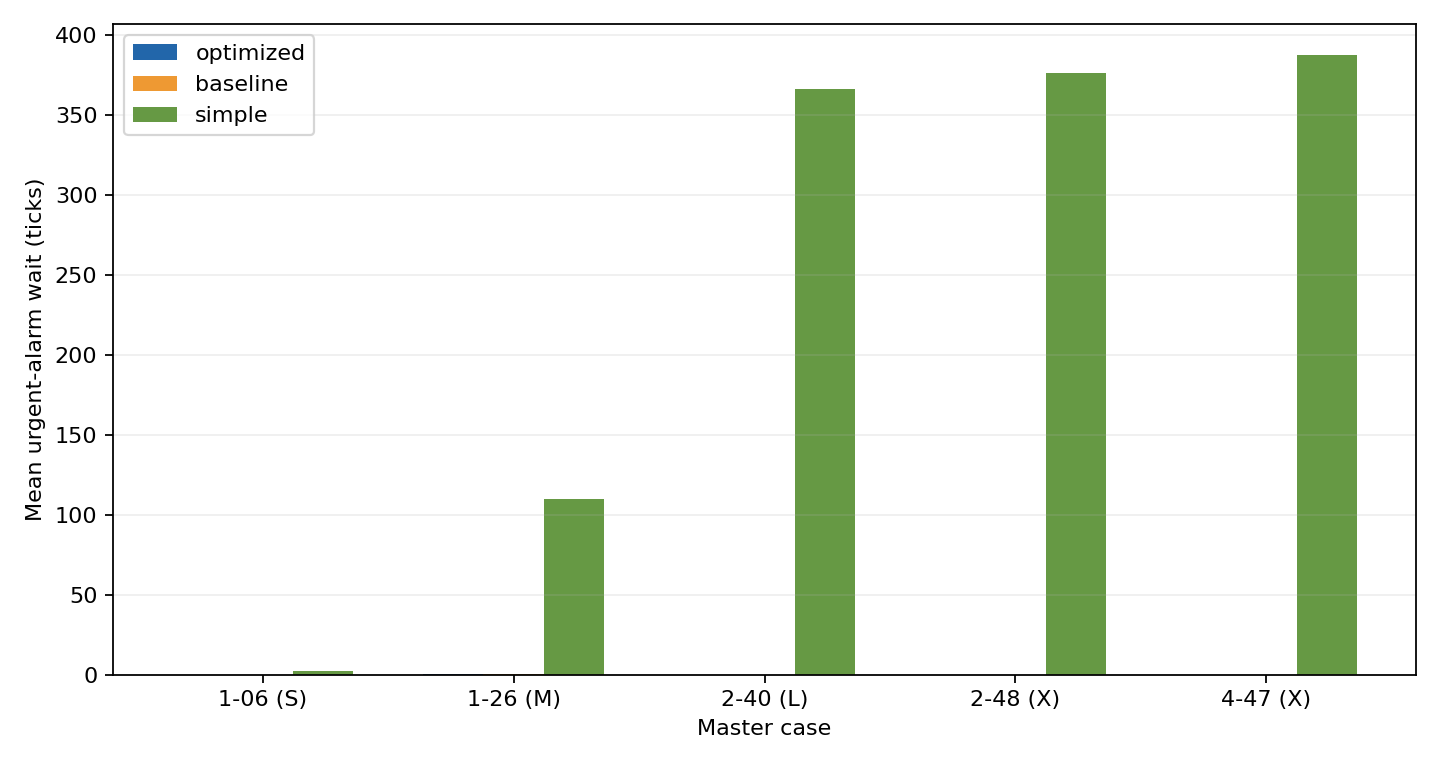
\includegraphics[width=0.62\textwidth]{campaign-urgent-wait.png}
\caption{Mean wait of urgent alarms in the five campaign cases under the three policies (from \cs{results/plots}).}\label{fig:camp}
\end{figure}

%%%%%%%%%%%%%%%%%%%%%%%%%%%%%%%%%%%%%%%%%%%%%%%%%%%%%%% 8
\section{Screenshots and interface}\label{sec:ui}
For the bonus the group built \emph{The Lifeline Gazette}, a local web interface in the style of a newspaper (\cs{python -m frontend --master MASTER}). It uses only the standard library on the server and plain HTML, CSS and JavaScript in the browser, and reads all results from the endpoints of the backend; the pages compute no decisions themselves.
Maps are schematic because the data have no coordinates. The Daily Edition (Figure~\ref{fig:ui1}) shows one campaign day with route, load, dispatches and the rescue timetable; Week in Review (Figure~\ref{fig:ui2}) shows the totals and the comparison with the baselines; the Map Room (Figure~\ref{fig:ui3})
lets the user close roads or waves and change the routing method; the Works Desk offers G live with every method.

\begin{figure}[t]
\centering
\begin{subfigure}{0.32\textwidth}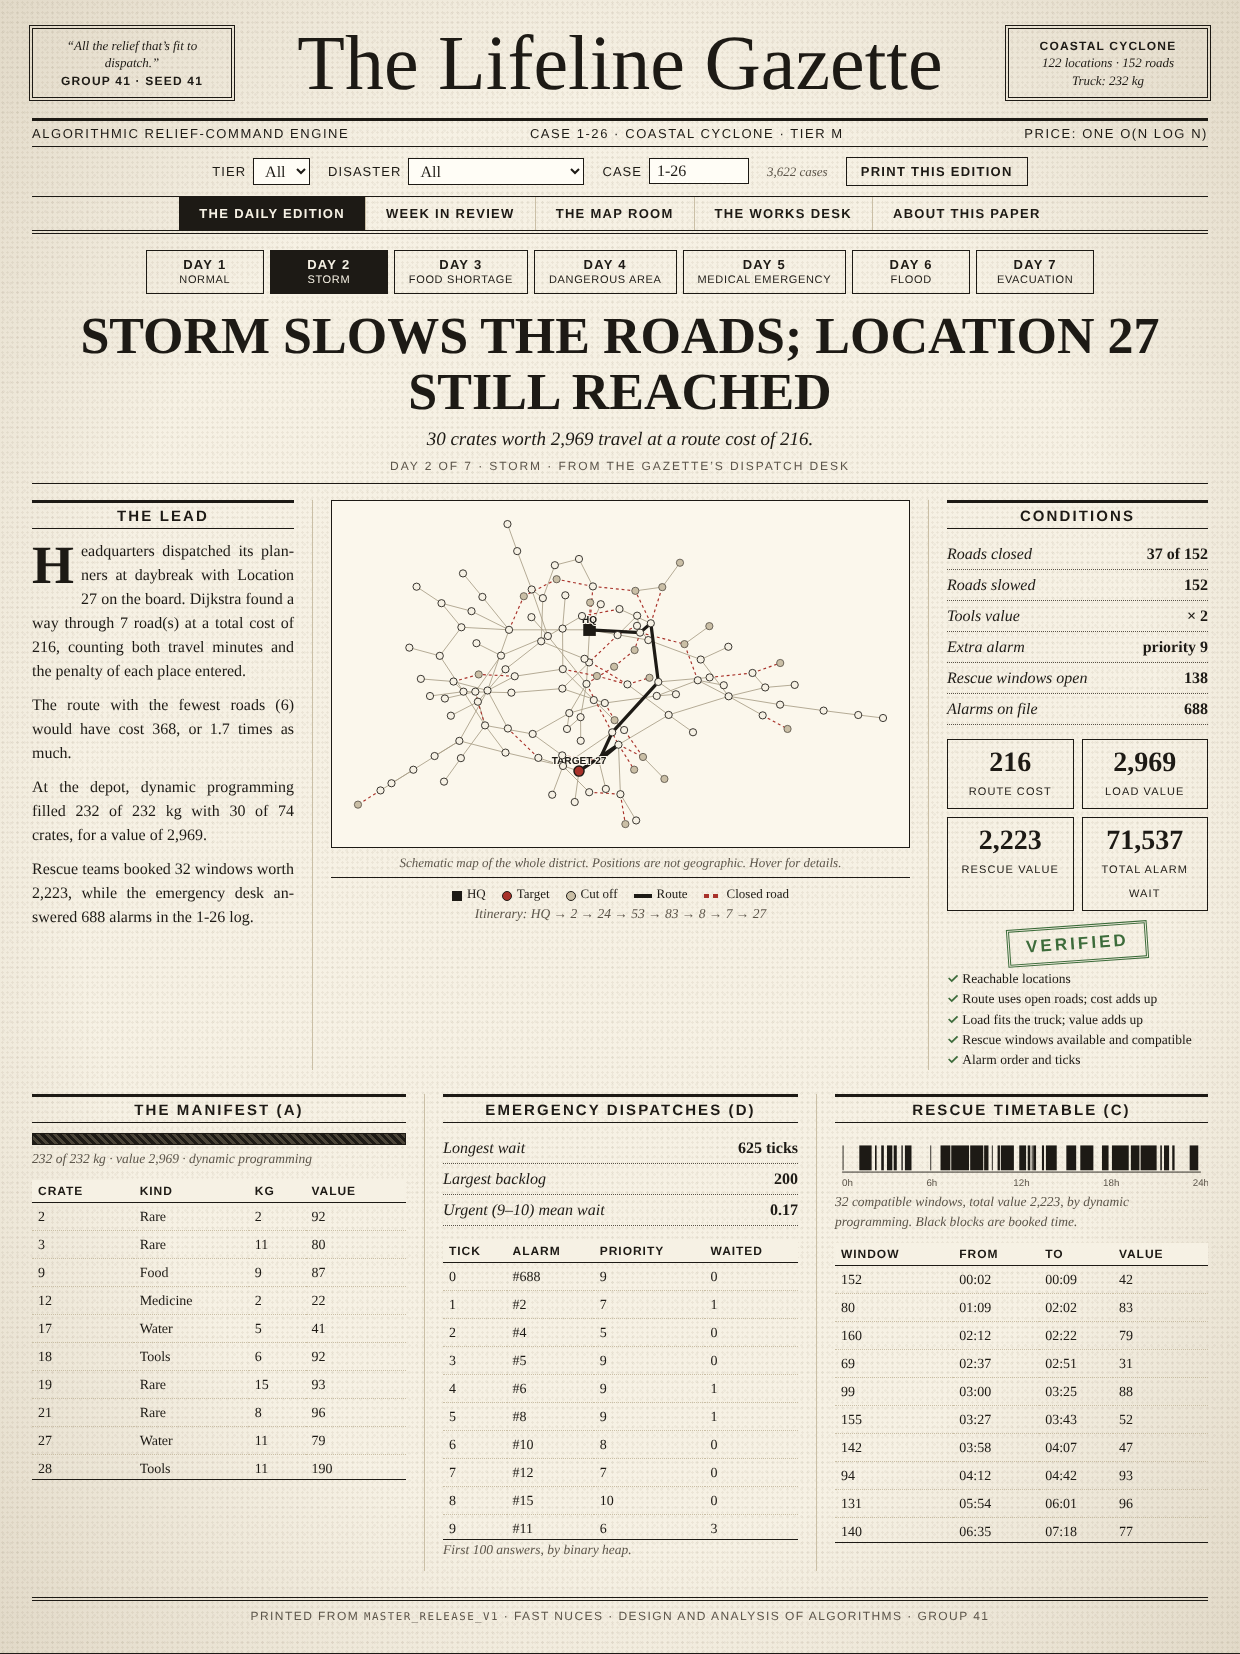
\includegraphics[width=\linewidth]{gazette-daily-edition.png}\caption{Daily Edition, one campaign day.}\label{fig:ui1}\end{subfigure}\hfill
\begin{subfigure}{0.32\textwidth}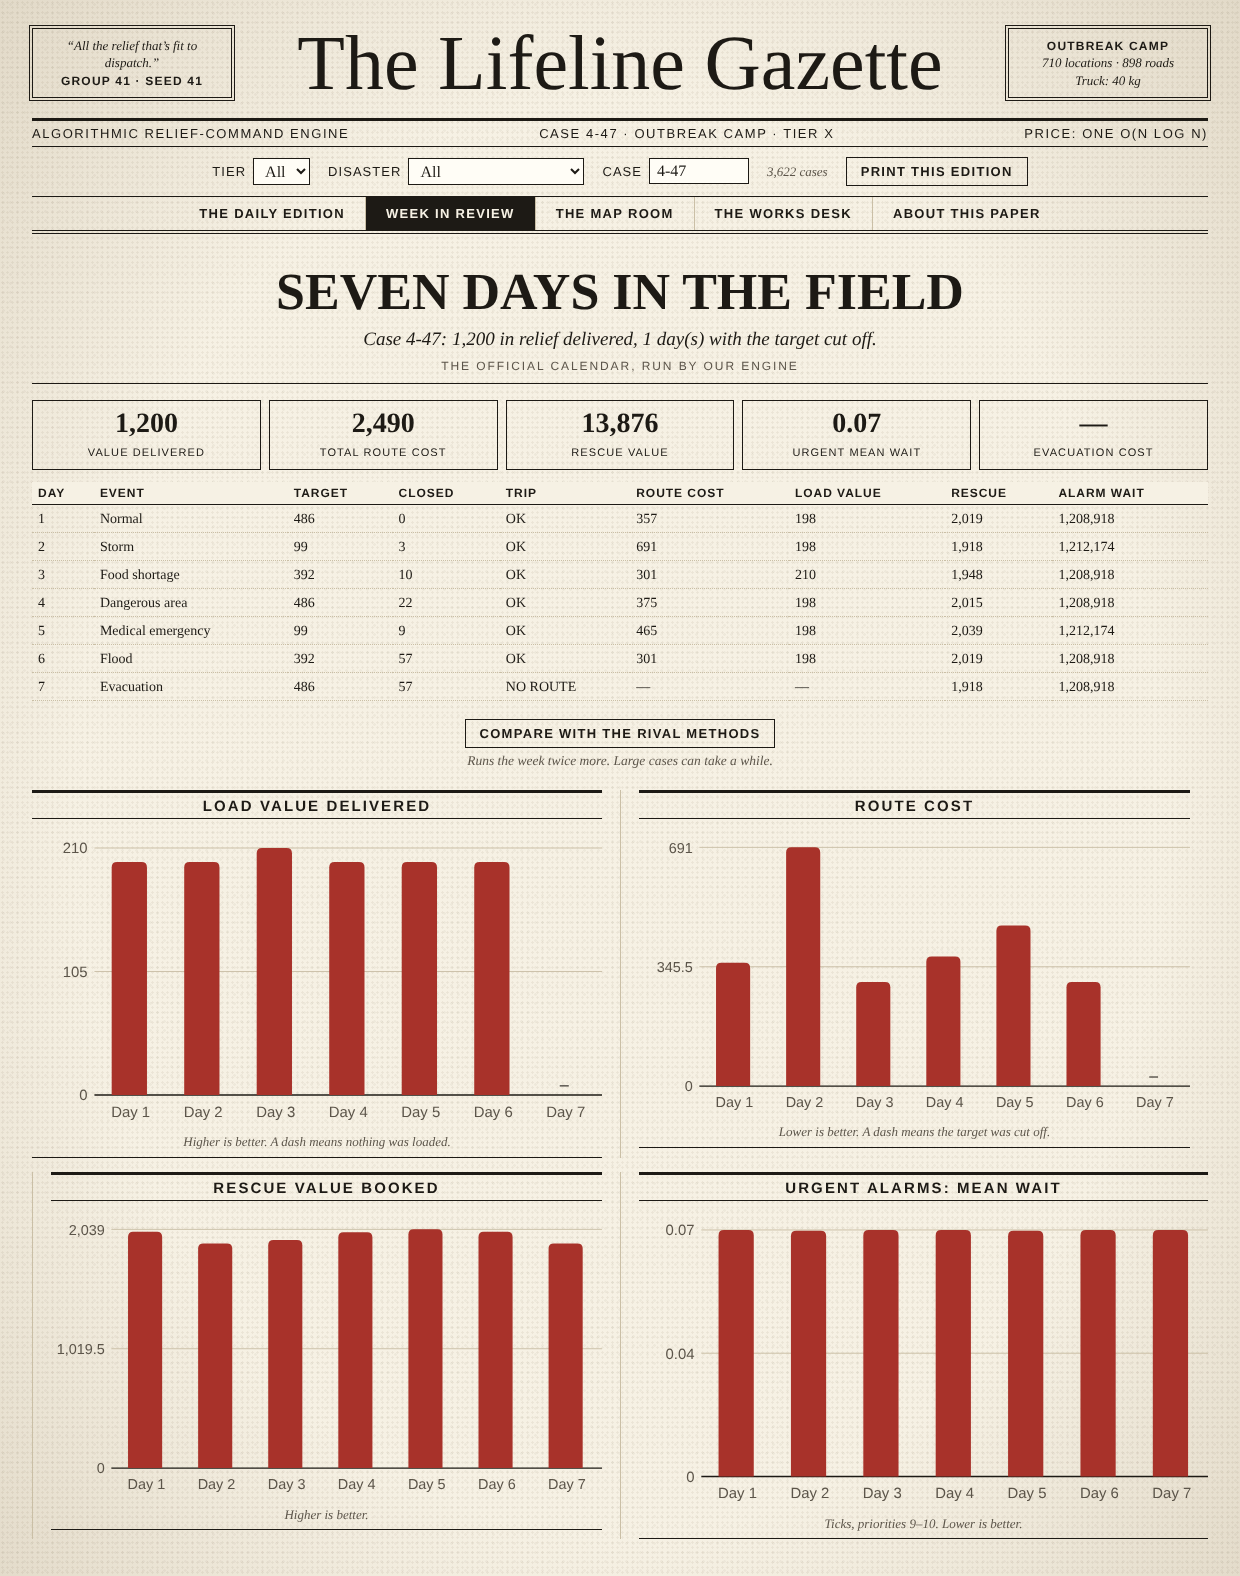
\includegraphics[width=\linewidth]{gazette-week-in-review.png}\caption{Week in Review, with the baseline comparison.}\label{fig:ui2}\end{subfigure}\hfill
\begin{subfigure}{0.32\textwidth}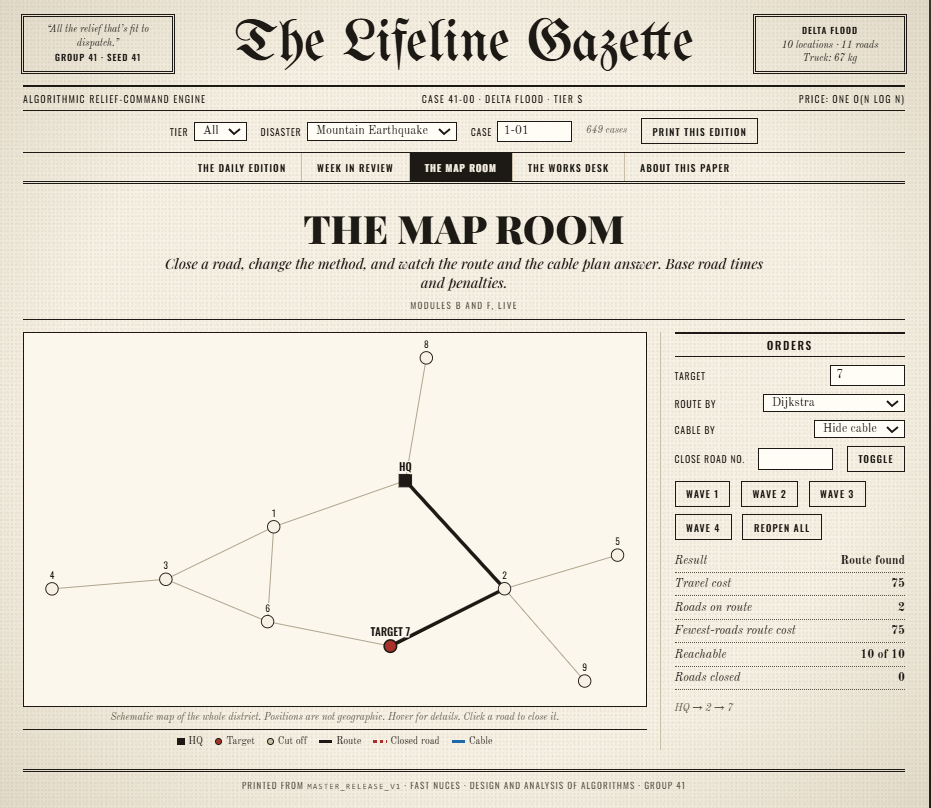
\includegraphics[width=\linewidth]{gazette-map-room.png}\caption{Map Room, case 1-01: Dijkstra from HQ to target 7 costs 75 over two roads.}\label{fig:ui3}\end{subfigure}
\caption{Three pages of the interface (screenshots of the running program).}
\end{figure}

%%%%%%%%%%%%%%%%%%%%%%%%%%%%%%%%%%%%%%%%%%%%%%%%%%%%%%% 9
\section{Recommendation to the lead designer}\label{sec:rec}
The group recommends the following engine, with the assumption under which each choice stands and the measurement that tells when it stops being right.
\begin{itemize}
\item \textbf{A: ship the DP.} Greedy is within 0.2\,\% of the optimum on tier M and 0.01\,\% on tier L, and 800 times faster, but loses 44\,\% on the trap-47 crates. A truck is loaded once a day and the DP costs seconds, so a hostile case is not worth the risk. It stands while $n\cdot\min(W,\text{total weight})$ stays below about $5\cdot10^7$; compute it before the run and fall back to greedy above it.
\item \textbf{B: ship heap Dijkstra} with BFS for reachability. It assumes positive costs and sparse maps; validation rejects negative values. \textbf{F: ship Kruskal} with Prim as a check.
\item \textbf{C: greedy for the count, the DP for the value.} Greedy is optimal for the count, but loses 16 to 28\,\% of the value on average. It assumes that windows compete only for time; with a second shared resource the compatibility test is wrong.
\item \textbf{D: ship the binary heap.} It assumes more alarms than releases (1.2 to 1.8 per tick against one), so the backlog grows; the maximum backlog reported in each plan tells when a scan of a few dozen alarms would do (the two were close at 250 alarms).
\item \textbf{G: ship the bottom-up DP.} For the drum, greedy is the fallback when $L^2$ is too large. A chain of 2\,000 matrices has about $1.3\cdot10^{9}$ candidates and was not run.
\end{itemize}

\textbf{The three failure modes of the whole engine that worry the group most (ranked).}
\begin{enumerate}
\item \textbf{A method that becomes too slow on a bigger case.} The A table has $nW$ cells, the chain DP is cubic (13~s at 640 matrices, an estimated 7~min at 2\,000) and the plain baselines of C and D are DNF at 200\,000 windows and 256\,000 alarms.
A deadline only tells after the time is gone, so the cost formulas should be evaluated before the run and the fallback chosen from them.
\item \textbf{Dispatch on stale or invalid road data.} Dijkstra is wrong for negative costs, and a closure that is not refreshed sends a vehicle to a location that is cut off. In the campaign days 6 and 7 cut off the destination in every case. Trap 48 shows that choosing the method by habit (fewest roads) costs 5.3 times the cheapest route.
\item \textbf{Low-priority alarms that wait without bound.} When more alarms arrive than can be answered, the urgency order protects priority 9 and 10 alarms (0.07 to 0.17 ticks of mean wait in the campaign), but the rest queue up: the longest wait was 2\,023 ticks for 2\,258 alarms in one tier L case, and the mean wait of all alarms is no better than under FIFO.
The remedy is capacity, not a cleverer queue; the backlog should be reported in every plan.
\end{enumerate}

%%%%%%%%%%%%%%%%%%%%%%%%%%%%%%%%%%%%%%%%%%%%%%%%%%%%%%% 10
\section{Limitations and conclusion}\label{sec:limits}
\textbf{Limitations.} (1) The code is pure Python: a DP cell costs about 85~ns, the chain DP 0.31~$\mu$s per candidate; larger sizes than those listed were not run. (2) All timings come from two laptops with unverified power state; some IQR values are large (for example the memoised chain at $n=40$)
and rounds 2 and 4 of A and D are from the slower run, so absolute times are weaker than operation counts and quality numbers. (3) Pools join consecutive cases; they keep the structure of real data but not a single big scenario, and B and F use nested prefixes of one graph.
(4) The quality results are tied to the sampled cases (62 per module) and to the shape of the master data: the good result of the drum greedy depends on concave-looking price tables. (5) The reading of the statement is ours where it is silent: pool capacity, the tie rule among equal-value loads and the meaning of ``master order''.
(6) The ten-bucket queue, branch and bound, array Dijkstra and the $O(n\log n)$ chain algorithm of Hu and Shing were not implemented. (7) The commit history of A and D does not prove that the predictions were committed before the results (Section~\ref{sec:exp}).

\textbf{Conclusion.} For every module the measured growth follows the theoretical class, and the cheap greedy rules turned out to be the interesting ones: nearly optimal on the real data for the knapsack on tiers M and L and for the drum cut, but clearly wrong on the trap-47 crates and on the value of windows.
Theory told the group what to expect in each experiment, and the predictions were mostly right; the misses were where a laptop changed speed or where the data were friendlier than the worst case.
What the group learned is mostly practical: that an independent reference and planted faults find bugs that unit tests written by the same person miss (the CRLF problem is one example), that a tie rule has to be written down before two methods can be compared, and that a measurement protocol is only worth something if it is applied on a machine whose state is known.

%%%%%%%%%%%%%%%%%%%%%%%%%%%%%%%%%%%%%%%%%%%%%%%%%%%%%%% 11
\section{Work division}\label{sec:work}
Iteration 1 (data) and Iteration 2 (engine) are listed separately. The Iteration 1 rows follow the history of the repository.
\begin{table}[!ht]
\centering\small
\caption{Contribution of each member.}\label{tab:work}
\begin{tabularx}{\textwidth}{@{}>{\raggedright\arraybackslash}p{2.3cm}>{\raggedright\arraybackslash}p{1.5cm}XX@{}}
\toprule
Member & Iteration & Modules, code and data & Tests, experiments and report sections\\
\midrule
Ayna Khan (24I-0097) & 1 & generator core and pipeline, crates, safety rations, claims, radio logs, workbook writer; proposal & text validation checks and the test runner; proposal\\
 & 2 & A (inventory), D (queue), merge sort, measurement harness & tests and fault injection of A and D, runs and analysis (rounds 1 to 4), prediction log of A and D; report 3.1, 3.2, parts of 6\\
\addlinespace
Dur E Adan (24I-3037) & 1 & graph generator (networks, waves, targets, trap 48), tour sensors & route validation checks, test-case maker, approach parts 1 and 4, \cs{members.txt}, \cs{repository.txt}\\
 & 2 & C (rescue), G (chains and cuts), the Lifeline Gazette interface & tests and fault injection of C and G, runs and analysis, prediction log of C and G, interface tests; report 3.3, 3.4, 5, 8, parts of 6\\
\addlinespace
Hamza Sardar (24I-0089) & 1 & windows and alarms generator, the dataset \cs{cases.xlsx}, validator engine and exact checks & validation report, planted-objects approach note\\
 & 2 & B (routes), F (network), loader and validation, campaign coordinator, CLI and local API & tests and fault injection of B and F and of the campaign, runs and analysis, prediction logs of B, F and campaign; report 3.5, 4, 7, parts of 6\\
\bottomrule
\end{tabularx}
\end{table}
Sections 1, 2, 9 and 10 of this report were written and checked by the three members together.

%%%%%%%%%%%%%%%%%%%%%%%%%%%%%%%%%%%%%%%%%%%%%%%%%%%%%%% refs
\begin{thebibliography}{9}\small
\bibitem{clrs} T.\,H. Cormen, C.\,E. Leiserson, R.\,L. Rivest, C. Stein, \emph{Introduction to Algorithms}, 4th ed., MIT Press, 2022 (knapsack DP, heaps, merge sort, activity selection, matrix-chain multiplication, rod cutting, Dijkstra, Bellman-Ford, Kruskal, Prim).
\bibitem{kt} J. Kleinberg, E. Tardos, \emph{Algorithm Design}, Pearson, 2005 (interval scheduling and weighted interval scheduling).
\bibitem{hs} T.\,C. Hu, M.\,T. Shing, Computation of matrix chain products, \emph{SIAM Journal on Computing} 11 (1982) and 13 (1984).
\bibitem{mt} S. Martello, P. Toth, \emph{Knapsack Problems: Algorithms and Computer Implementations}, Wiley, 1990 (greedy ratio rule and its worst cases).
\bibitem{dij} E.\,W. Dijkstra, A note on two problems in connexion with graphs, \emph{Numerische Mathematik} 1 (1959) 269--271.
\bibitem{kru} J.\,B. Kruskal, On the shortest spanning subtree of a graph and the traveling salesman problem, \emph{Proc. AMS} 7 (1956) 48--50.
\bibitem{tar} R.\,E. Tarjan, Efficiency of a good but not linear set union algorithm, \emph{Journal of the ACM} 22 (1975) 215--225.
\bibitem{stmt} Course staff, \emph{LIFELINE project statement}, and the master dataset \cs{master\_release\_v1}, 2026.
\end{thebibliography}

\end{document}
